\documentclass[a4paper,fleqn,usenatbib,useAMS]{mnras}

\usepackage{graphicx}	% Including figure files
\usepackage{amsmath}	% Advanced maths commands
\usepackage{amssymb}	% Extra maths symbols
\usepackage{multicol}        % Multi-column entries in tables
\usepackage{bm}		% Bold maths symbols, including upright Greek
\usepackage{pdflscape}	% Landscape pages
\usepackage{IEEEtrantools} % for stacked equations

\newcommand{\numax}{\ensuremath{\nu_{\textrm{max}}}}
\newcommand{\dnu}{\ensuremath{\Delta\nu}}
\newcommand{\teff}{\ensuremath{T_{\textrm{eff}}\:}} 
\newcommand{\kep}{\ensuremath{Kepler}}
\newcommand{\pdet}{\ensuremath{P_{\rm det}\:}}

\newcommand{\bibtex}{\textsc{Bib}\!\TeX} % bibtex. Not quite the correct typesetting, but close enough

\usepackage[T1]{fontenc}
\usepackage{ae,aecompl}
%\usepackage{newtxtext,newtxmath}  % new version
\usepackage{txfonts}  % old version

\title[TRG]{TESS Asteroseismic Predictions for Red Giants using Machine Learning}

\author[M. Schofield et al.]{M. Schofield$^{1, 2}$\thanks{E-mail: mxs191@bham.ac.uk}, G. R. Davies$^{1, 2}$, W. J. Chaplin$^{1, 2}$, M. F. Randrianandrasana
\\
% List of institutions
$^{1}$Department of Physics and Astronomy, the University of Birmingham, Birmingham B15 2TT, UK \\
$^{2}$Stellar Astrophysics Centre (SAC), Department of Physics and Astronomy, Aarhus University, Ny Munkegade 120, DK-8000 Aarhus C, Denmark}


%\thanks{Contact e-mail: \href{mailto:mxs191@bham.ac.uk}{mxs191@bham.ac.uk}}\thanks{Present address: Department of Physics and Astronomy, the University of Birmingham, Birmingham B15 2TT, UK}



\date{Last updated 2017 May 31; in original form 2017 May 31}
\pubyear{2018}

\begin{document}
\label{firstpage}
\pagerange{\pageref{firstpage}--\pageref{lastpage}}
\maketitle

\begin{abstract}
{\it Summary}: This paper presents a method to predict Red Giant mode detectability with TESS, using the Machine Learning algorithm Classification. It requires only the global parameters \dnu, \numax, the stellar magnitude and length of observation. \newline
{\it Method}: Lightcurves for \kep \ stars with fitted radial mode frequencies were used to generate equivalent TESS lightcurves. The lightcurves were cut down, \kep \ white noise was removed, the bandpass was adjusted, and TESS white noise was added. A detection test was run on the observed modes in these 'TESS-like' lightcurves. Classifiers were then used to predict mode detectability with TESS based upon the global asteroseismic parameters \numax \ and \dnu, as well as the stellar magnitude.\newline
{\it Application}: By changing only the length of dataset and instrumental noise level, this tool can make predictions for any future mission such as K2, PLATO or CoRoT. This is therefore an ideal tool for target selection.
\end{abstract}


\section{Introduction}

Satellites such as $Kepler$ have allowed asteroseismology of solar-like and Red Giant stars to advance rapidly since the last century \citet{chaplin_asteroseismology_2013}. Power spectra can now be resolved to detect individual modes of oscillation in Main Sequence and Red Giant stars (\citet{lund_standing_2017} and \citet{davies_asteroseismology_2016}, respectively).

Future space missions such as TESS \citep{ricker_transiting_2014}, K2 \citep{howell_k2_2014}, CoRoT \citep{baglin_corot:_2006} and PLATO \citep{rauer_plato_2014} will add to our understanding of stellar structure and evolution. These missions will provide a large amount of high-precision data. More than ever, the field of stellar astrophysics will require tools to perform big-data analysis \citep{kremer_big_2017}. 

%In order to select asteroseismic targets for these missions, the detectability of solar-like oscillations inside these stars needs to be estimated.

One of the tools than can be used to handle this larger amount of data is Machine Learning. In this work, Machine Learning was used to create a TESS target selection function using the set of $Kepler$ Red Giant stars from \citet{davies_asteroseismology_2016}. This publicly-available algorithm can be used to select targets for any future space mission.

In most situations, Machine Learning is used to solve problems in one of two ways; Supervised or Unsupervised Learning. Supervised Learning involves problems where there is a known result. 

Supervised Learning has been used to classify types of variable star using previously labelled data (\citet{nun_supervised_2014}, \citet{elorrieta_machine_2016}). This previously labelled data is known as training data: this is used to train the Machine Learning algorithm. In the problem of variable stars, lightcurves that had already been classified were used to train the algorithm (this is the training dataset). This algorithm was then used to classify the lightcurves of unidentified stars (this is known as the testing dataset).

In Unsupervised Learning, there are no known results (labels). The aim of Machine Learning in this case would be to find trends between variables. This could be used to identify similar stars by analysing their lightcurves without using previously labelled data (for example, \citet{valenzuela_unsupervised_2018}).

The aim of this work is to use Machine Learning to make predictions about mode detection probability (\pdet). In this case, \pdet is a known label, so this is a Supervised Learning problem\footnote{https://machinelearningmastery.com}.

Within Supervised Learning, two common algorithms are that are used are Classification and Regression. In Regression, the relationship between variables is interpreted using a measure of uncertainty (such as using $\chi^{2}$ tests). Models are fitted using the independent data, and uncertainty is measured. The models are then improved by reducing this uncertainty. Note that regression is used when the label is continuous. For example, predicting the magnitude of a star is a problem suited to regression, as a star can have any magnitude.

Conversely, Classification algorithms work by assessing similarity\footnote{http://www.simafore.com}. In Classification, the training set is separated into groups based on the similarity of the data. The more information that was gained by splitting the data, the better. For example, if the problem were to separate Red Giant stars from Main-Sequence stars, a star could be classified as either a Red Giant (1), or not a Red Giant (0). For example, having a Luminosity above $\sim10L_{\odot}$ would be a strong indicator that the star was a Red Giant, so the data could be separated into groups here. The Classifier would continue to separate the dataset until the Red Giant and Main Sequence samples were distinct. This is not the only problem where Classification can be used on Red Giant stars (\citet{ness_cannon_2015}, \citet{wu_mass_2017}).

In this work, individual fitted modes from \citet{davies_asteroseismology_2016} were used to make asteroseismic predictions for TESS. By separating the targets into those with detected modes and those without, Machine Learning was used to select targets for future observation. Section \ref{sect: dataset} describes how the timeseries of every star was treated before transforming it to a power spectra. Section \ref{sect: det_test} then goes on to describe the detection test that was run on every fitted mode. Every mode was grouped into observed (1), or unobserved (0).

Lastly, Section \ref{classifier} describes the classification of stars into a group with detected modes, and a group without. This was done by giving a Supervised Classifier information on every target: the frequency of maximum solar-like amplitude \numax, the large separation between modes of the same angular degree \dnu, the stellar magnitude, and which modes were detected inside the star. 70\%???? of the stars were used to train the Classifier; 30\%????? of the sample was kept to test the algorithm. The Classifier recognised patterns between the variables in the training set, and made predictions on the testing set with a ?????????\% accuracy. 


\iffalse
\section{Transforming the lightcurves}
\label{sect: dataset}

Firstly, the timeseries data from \kep \ observations needed to be adjusted for a different satellite and mission. This could either be done in the time or frequency domain. Both methods were tested and compared. The time domain method was chosen to transform the lightcurves, and was used in the rest of this work.

Several different adjustments needed to be made to the \kep \ data. One difference between the missions is the length of observation. The \kep \ mission observed for 4 years, while TESS' nominal 2 year mission will observe stars for between 27 days to 1 year, according to the star's ecliptic latitude (Figure \ref{TESS field}). This distinction is made clear in the timeseries, see Figure \ref{ts plot}.

\begin{figure}
	\centering
	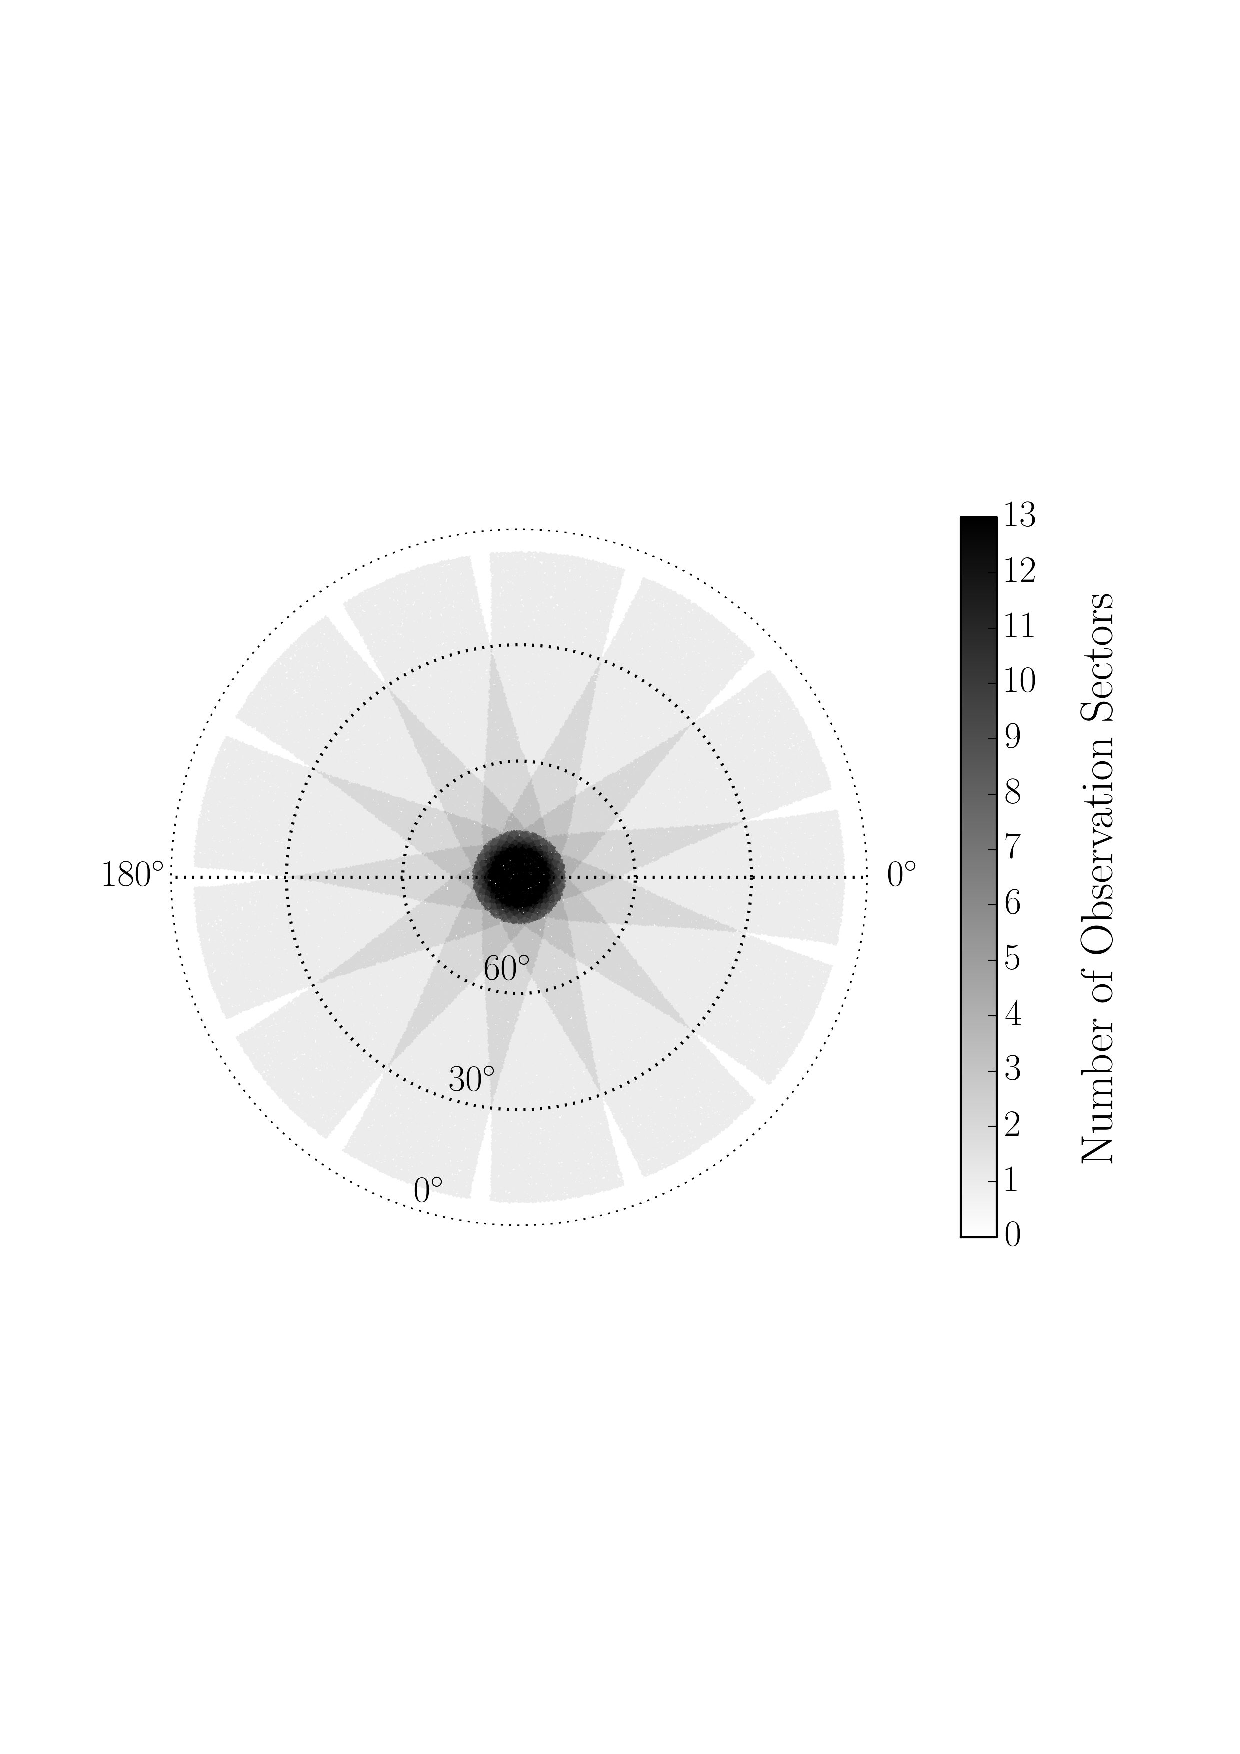
\includegraphics[scale=0.4]{cropped_TESSfield.pdf}
	\caption{TESS field of view, centred around the ecliptic pole. Each strip will be observed for 27 days before the satellite rotates. Image taken from \citet{campante_asteroseismic_2016}.}	
	\label{TESS field}
\end{figure} 

\begin{figure}
	\centering
	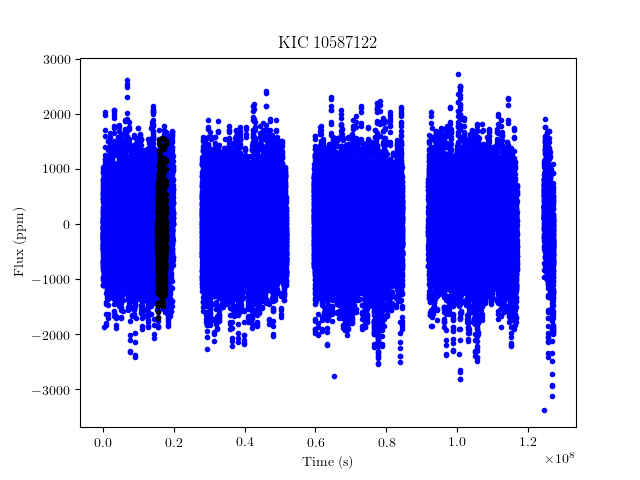
\includegraphics[scale=0.6]{timeseries_10587122}
	\caption{The 4-year long Power Spectra of KIC 10587122 is plotted in blue. Overplotted is the 27-day time segment with most coverage (the period with fewest gaps in the data). Reducing the length of observation this drastically will badly hamper mode detectability.}	
	\label{ts plot}
\end{figure} 

As well as reducing the dataset length, the bandpass that TESS will observe in is much redder than that of \kep, Figure \ref{bandpass}. This has the effect of reducing the amplitude of stellar signals (i.e the signal due to stellar granulation and oscillation). \citet{campante_asteroseismic_2016} found this bandpass correction to be 0.85.

\begin{figure}
	\centering
	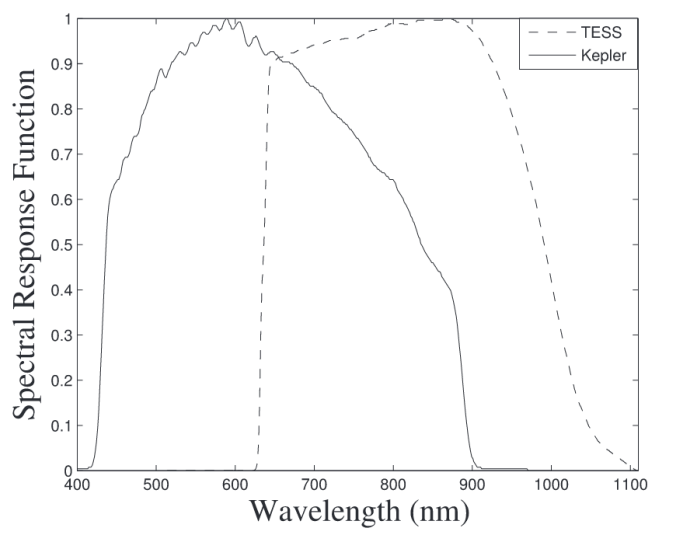
\includegraphics[scale=0.4]{bandpass.png}
	\caption{The bandpass of the $Kepler$ and TESS missions. TESS will observe at longer (i.e redder) wavelengths than $Kepler$. This will reduce the amplitude of oscillations and granulation, whilst the white noise level will by unaffected.}	
	\label{bandpass}
\end{figure} 

Thirdly, the instrumental noise level in \kep \ is different to the noise level in TESS. The noise level for the \kep \ satellite depends on the \kep \ magnitude of the star, $K_{p}$. The noise can be calculated using
\begin{equation}
\frac{10^{6}}{c} \times \sqrt{c+9.5 \times 10^{5}\Bigg(\frac{14}{K_{p}}\Bigg)^{5}} ,
\end{equation}
where
\begin{equation}
c = 1.28 \times 10^{0.4(12-K_{p})+7} ,
\end{equation}
from \citet{chaplin_predicting_2011}.

As well as subtracting this noise from the signal, instrumental noise from TESS needed to be added. This noise was estimated using the `calc noise' IDL procedure (from William Chaplin, private communication), which depends on the $I_{c}-$band magnitude of the star and the number of pixels in the photometric aperture used when observing the star. This is given by
\begin{equation}
N_{\rm aper} = 10 \times (n+10) , 
\end{equation}
where $n$ is
\begin{equation}
n = 10^{-5.0} \times 10^{ 0.4 \times (20-I_{\rm mag})} .
\end{equation}

These three adjustments - the length of observation, the bandpass, and the noise level - were performed in the time and frequency domains for comparison. The methods used are outlined in Figures \ref{ts flowchart} and \ref{fr flowchart}. The resulting Power Spectra are compared in Figures \ref{Power Spectra} and \ref{overplotted PS}. From these results, it was decided to add noise in the time domain, before transforming to frequency. 

After noise was added to the stars and power spectra were made, a detection test was run on every fitted mode of every star. 

\begin{figure}
	\centering
	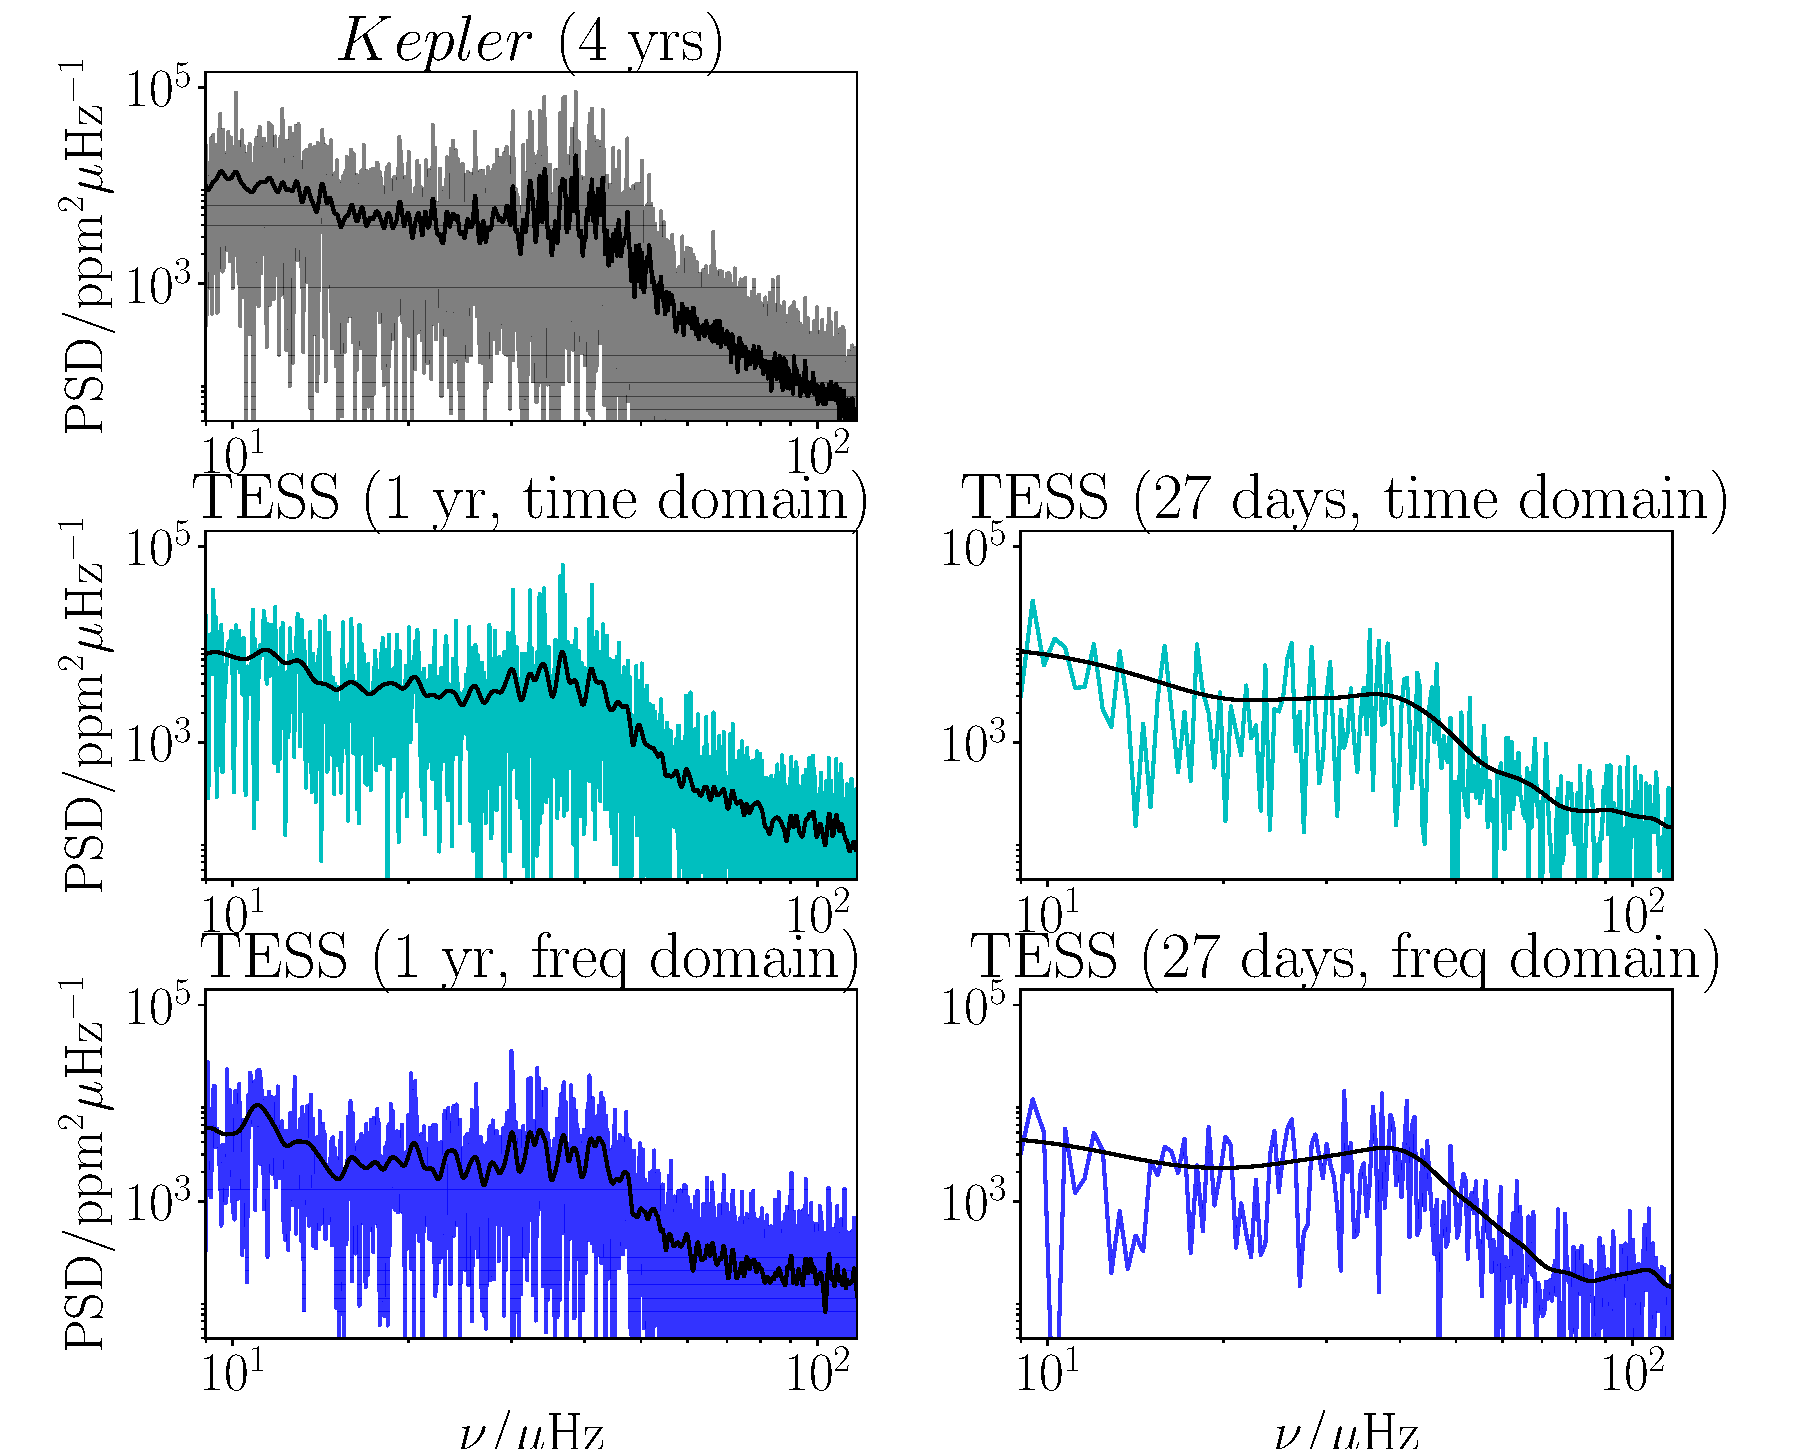
\includegraphics[scale=0.3]{diagnostic_plot1_modes}
	\caption{The Power spectra of KIC 10587122 is plotted five times. The original Power Spectra is plotted in grey. The power spectra after making the data look like TESS are plotted in blue. The data was transformed in the time domain (light blue) or frequency domain (dark blue). The left column shows 1 year of TESS observation (the maximum). The right column shows 27-days (the minimum). Based on this, the time series was chosen to transform the data in.}	
	\label{Power Spectra}
\end{figure} 
\begin{figure}
	\centering
	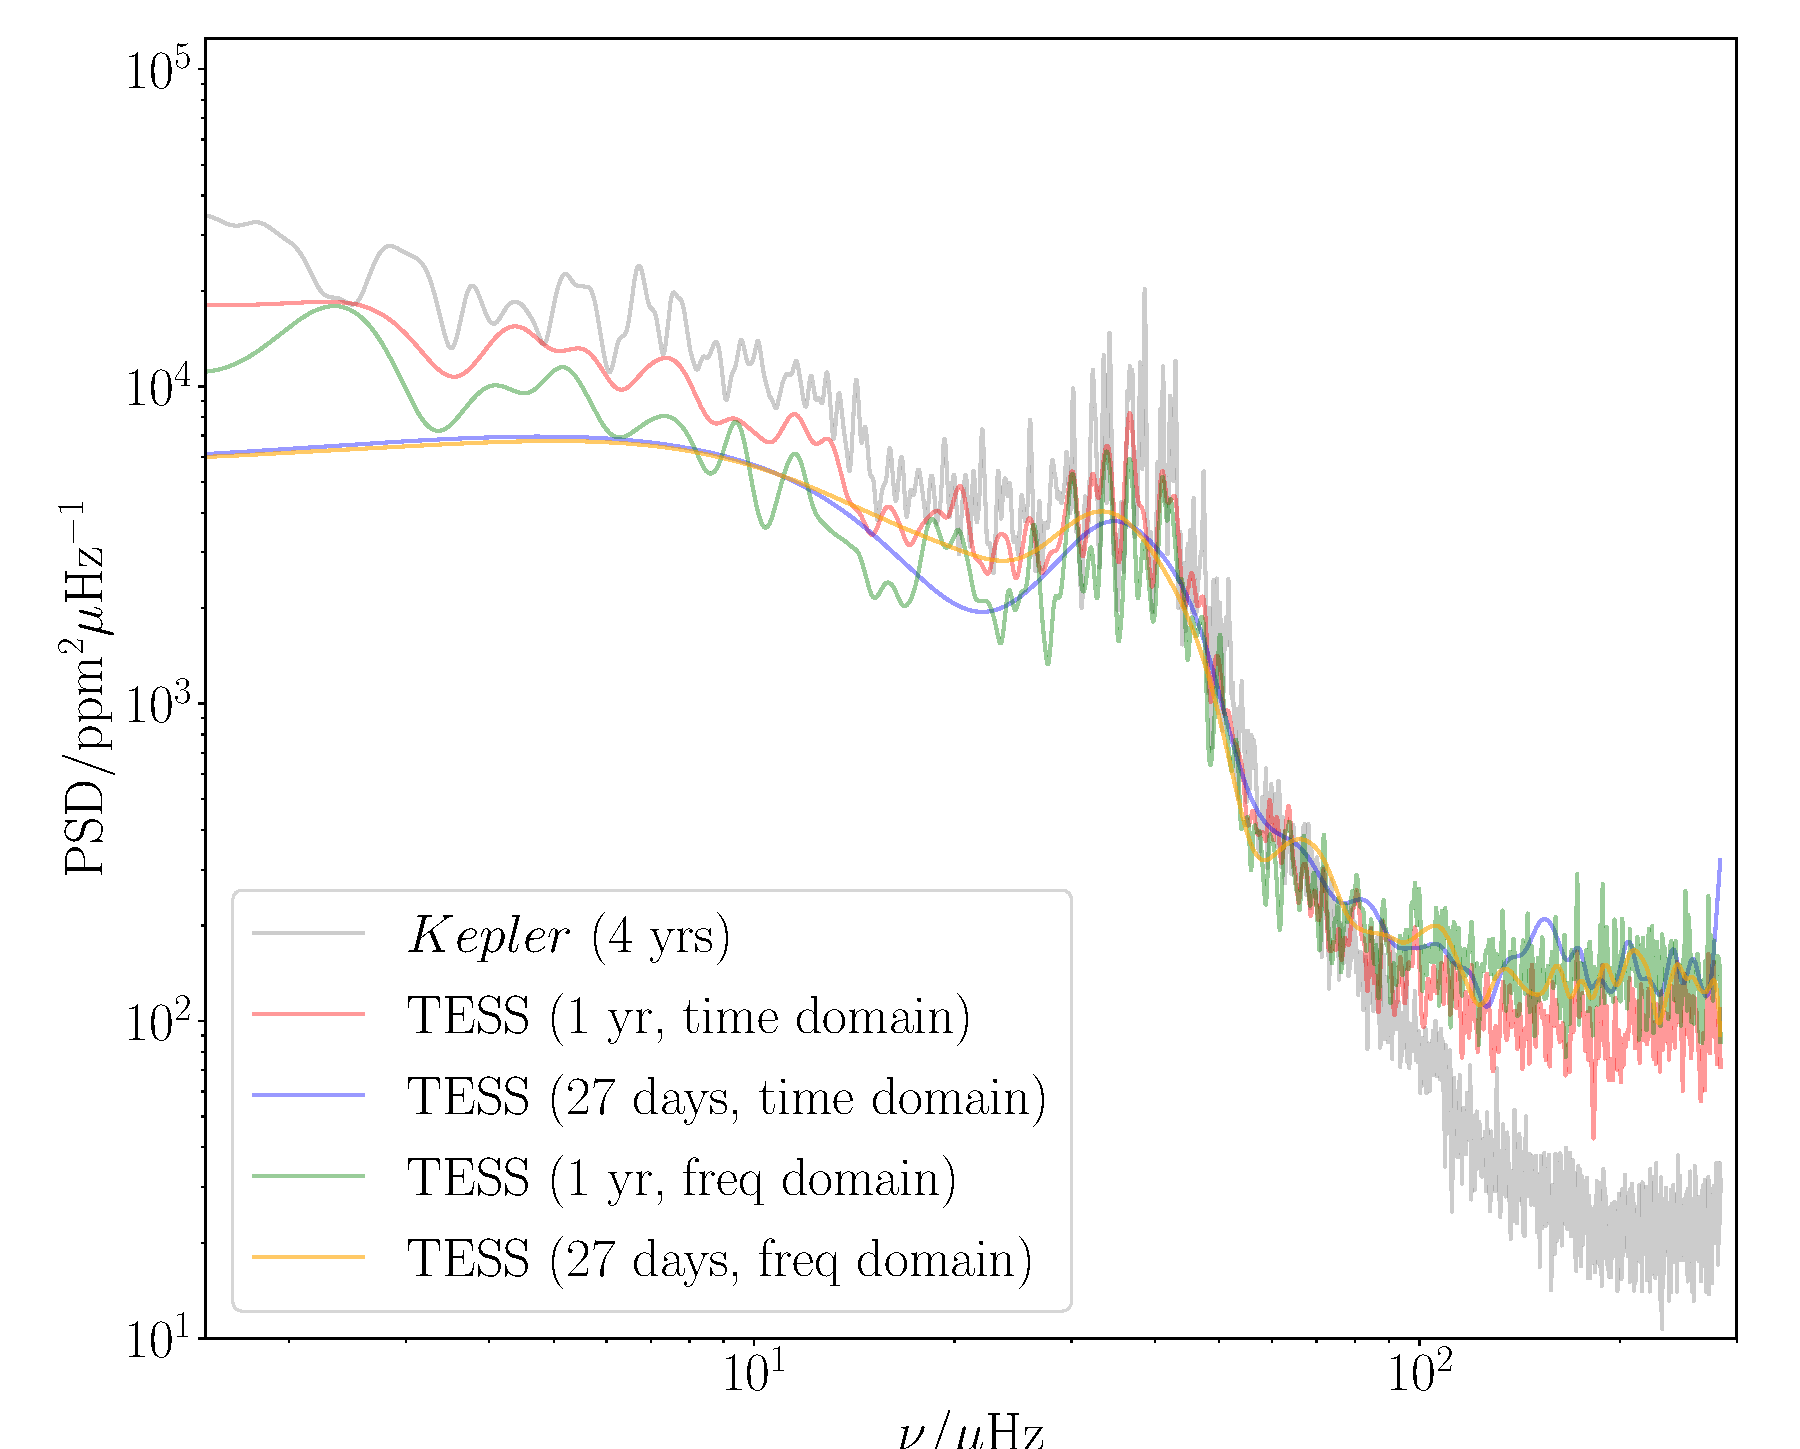
\includegraphics[scale=0.3]{diagnostic_plot2_full}
	\caption{The Power Spectra of KIC 10587122. The original power spectra is in grey. The data was transformed into TESS observation and overplotted. The transformation was done in the time and frequency domains for comparison. Based on this, the time series was chosen to transform the data in.}	
	\label{overplotted PS}
\end{figure} 


\onecolumn
\begin{figure}
	\centering
	\includegraphics[scale=0.5, trim={0 3cm 10cm 0}]{"TRG timeseries flowchart".pdf}
	\caption{Flow chart of the method to convert the data from \kep \ to TESS observations in the time domain.}	
	\label{ts flowchart}
\end{figure} 

\begin{figure}
	\centering
	\includegraphics[scale=0.5, trim={0 3cm 0 0}]{"TRG frequency flowchart".pdf}
	\caption{Flow chart of the method to convert the data from \kep \ to TESS observations in the frequency domain.}	
	\label{fr flowchart}
\end{figure}
\newpage
\twocolumn


\section{Detection Test}
\label{sect: det_test}

Section \ref{sect: dataset} described the method to transform the $Kepler$ lightcurves into TESS observations. A detection test was then run on the stars, to determine which modes were still visible with observation by TESS, and which could not be recovered.

First, a moving median from \citet{davies_asteroseismology_2016} was used. The width of the moving median is from the star's envelope width. This predicted envelope width was calculated as
\begin{equation}
\Gamma_{\rm env} = 0.66 * \numax^{0.88},
\end{equation}
from \citet{mosser_characterization_2012}. The moving median was used to interpolate between frequencies in the power spectrum. This moving median is a good estimate of the background of the star. It was divided out of the power spectrum to the get Signal-to-Noise spectrum,
\begin{equation}
\label{eq:snr}
{\rm SNR} = P/B.
\end{equation}
An example of this is shown in Figure \ref{snr}.

\begin{figure}
	\centering
	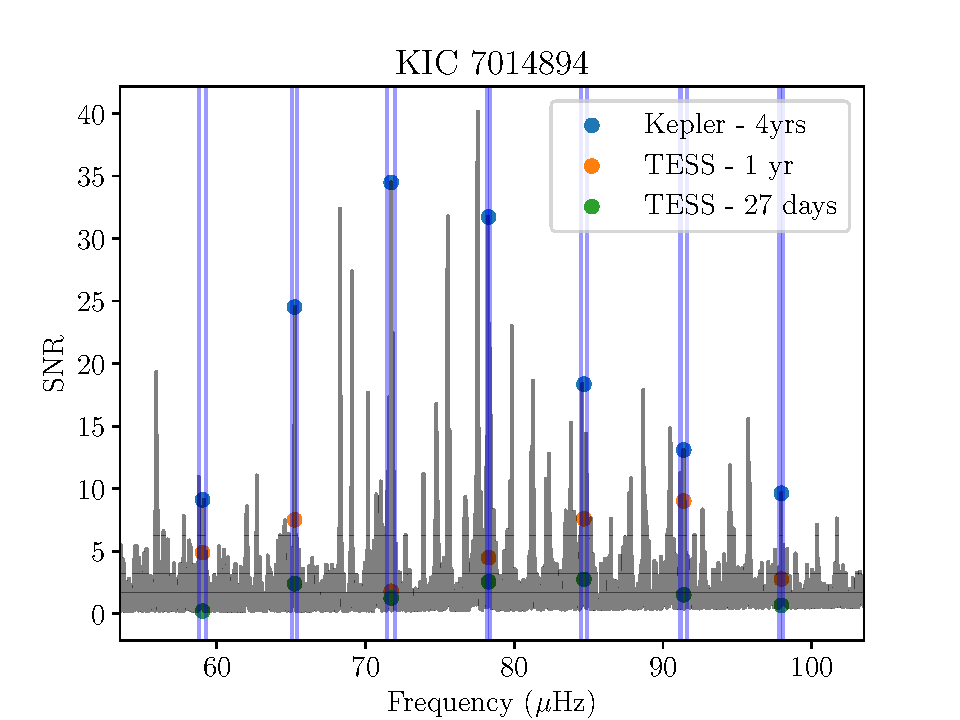
\includegraphics[scale=0.6]{plot4_SNR7014894.pdf}
	\caption{The power spectra of KIC 7014894 after background subtraction. The SNR value of every mode in the star was extracted from the SNR spectrum. The values for every mode in the original Kepler SNR are plotted in blue. The orange points are the SNR values after degrading the signal to 1 year of TESS observation. The green points are to 27 days.}	
	\label{snr}
\end{figure}

Once the SNR spectrum for the star was recovered, the SNR values of every mode were extracted. To ensure the correct SNR value was used, a window was fitted around each peak-bagged mode frequency. The size of the window was given as the linewidth of the mode. The highest value in the window was taken as the SNR of the mode. Figure \ref{modes} is an example of this process for one star. 

\begin{figure}
	\centering
	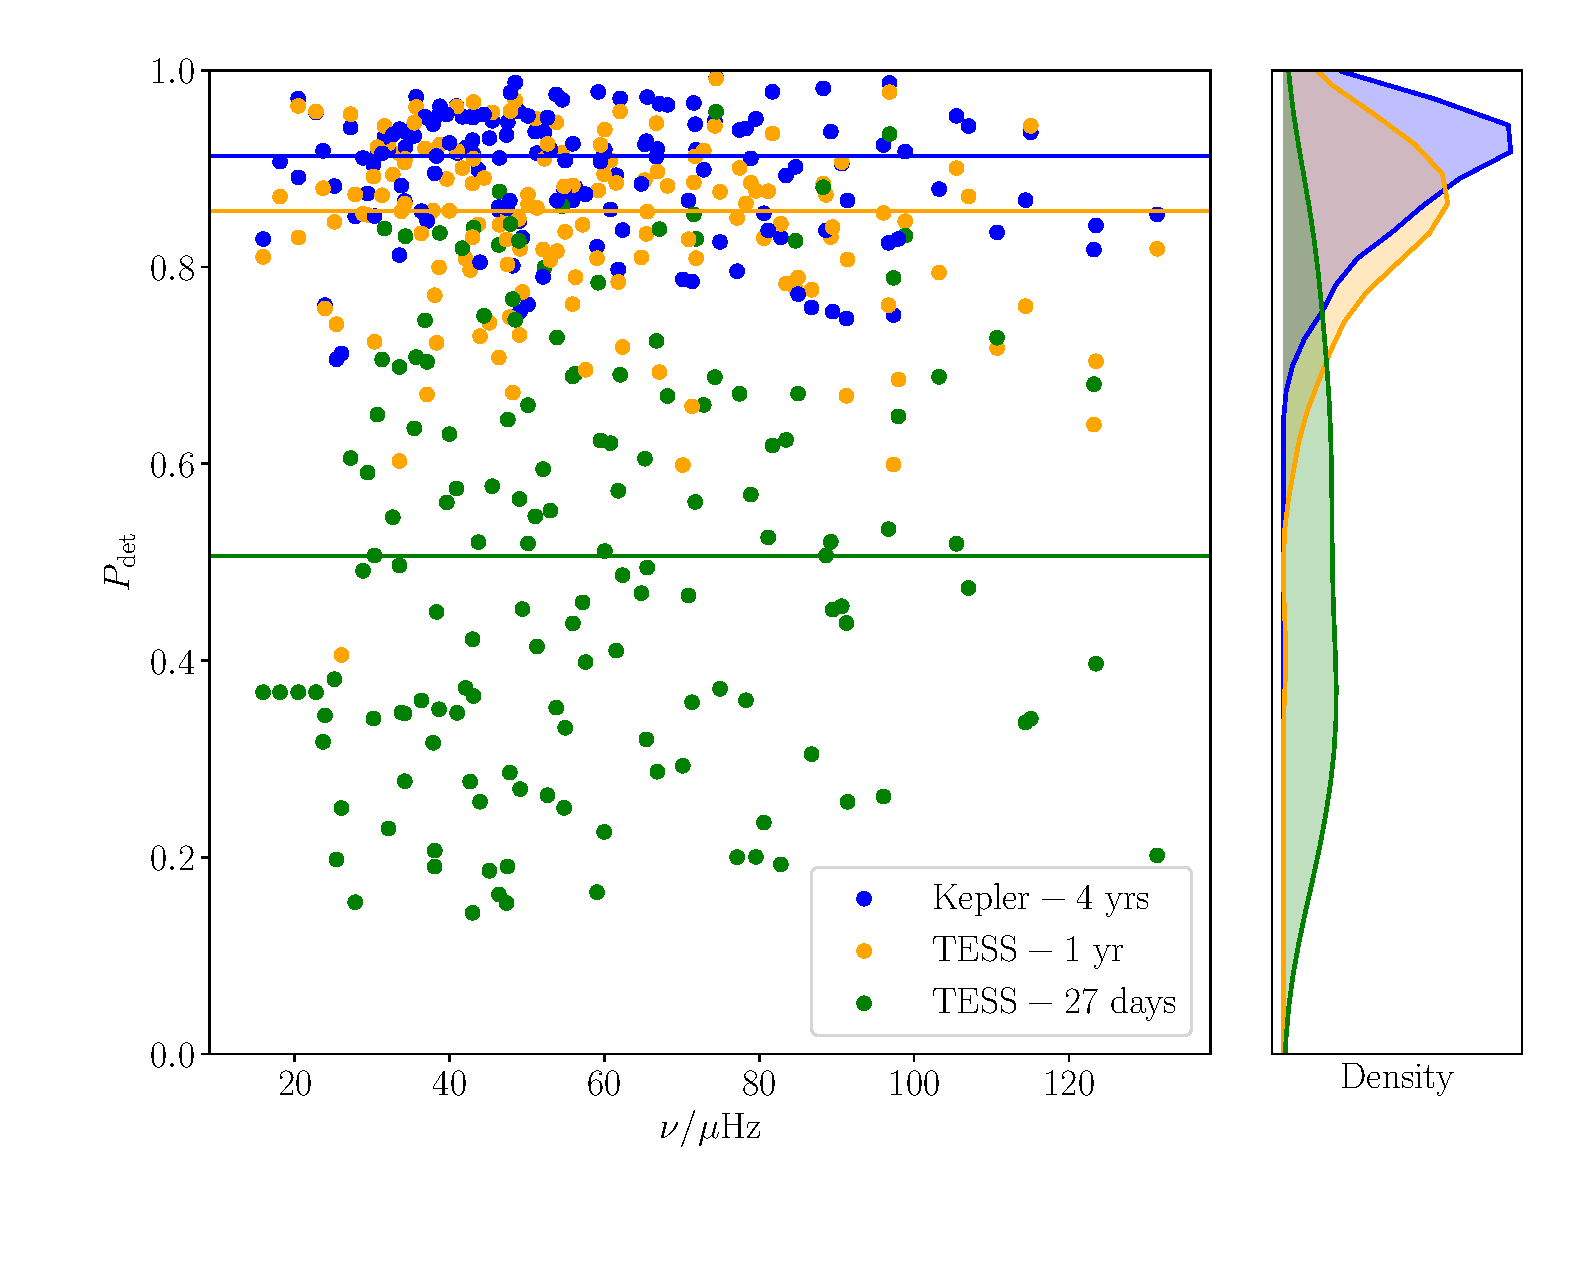
\includegraphics[scale=0.3]{DetTest_Diagnostic_plot3.pdf}
	\caption{A plot showing the result of the detection test, after running on every mode in 20 stars. The results of the original power spectra are plotted in blue. The results of 1 year of TESS observation are in orange. 27 days of TESS observation is in green. At this short an observation, detecting individual modes will be extremely difficult.}	
	\label{modes}
\end{figure}

Once all mode SNR values for the star were calculated, a detection test was run on every mode \citep{chaplin_predicting_2011}, \citep{campante_asteroseismic_2016}.

The probability $P$ that the SNR lies above some threshold ${\rm SNR_{thresh}}$ is
\begin{equation}
\label{eq:pdet}
P(\rm SNR \geq SNR_{thresh}) = \it p .
\end{equation}
A false-alarm probability $p$ of 1\% was set; there is a 99\% chance that the signal is due to solar-like oscillations, rather than noise. Equation \ref{eq:pdet} is solved for $\rm SNR_{thresh}$ by substituting $P$ with
\begin{equation}
\label{eq:prob}
P = \int_{x}^{\infty} \frac{e^{-x}}{\Gamma(N)} x^{N-1} dx .
\end{equation}
$\Gamma(N)$ is the Gamma function. The lower bound of Equation \ref{eq:prob} is set to $x=1+{\rm SNR_{thresh}}$. N is the number of frequency bins. The noise in this bin is assumed to follow $\chi_{2}$ $2n_{\rm bins}$ d.o.f statistics. 

Once $\rm SNR_{thresh}$ is found, Equation \ref{eq:prob} is solved again. This time it is solved for $P$ by setting $x=(1+{\rm SNR_{thresh}})/(1+{\rm SNR})$. Here, SNR is the observed Signal-to-noise Ratio calculated from Equation \ref{eq:snr}. This calculates the probability that the frequency spike was due to stochastic excitation in the convective envelope of the star.

This detection test was applied to every mode of every star in the 1000-star sample. Classification was then applied to this dataset. This is described in Section \ref{classifier}.


\section{Classification}
\label{classifier}

Section \ref{sect: dataset} describes how the lightcurves of every star were treated before a detection test was run on the modes in Section \ref{sect: det_test}. After this, Classification was applied to the stars to separate them into a suitable target list, and a list of stars that are not suitable for observation with TESS.

This could be done without using Machine Learning, although it takes much longer. In the age where datasets from missions such as MAST and Gaia \citep{gaia_collaboration_gaia_2016} exist, tools need to be developed to make use of the huge amount of information we now have on stars from across the sky.

\subsection{Preparing the data}
Firstly, the detection probabilities of every mode were taken from Section \ref{sect: det_test}. Each probability was changed to a 1 or 0 depending on if a detection was made. For each mode as observed by $Kepler$,
\begin{equation}
\label{eq:kep_class}
P_{\rm det, Kep} = \left\{ \,
    \begin{IEEEeqnarraybox}[][c]{l?s}
      \IEEEstrut
      1 & if \pdet $\geq$ 0.9 \, , \\
      0 & if \pdet $<$    0.9 \, .
      \IEEEstrut
    \end{IEEEeqnarraybox}
\right.
\end{equation}
Modes will be more difficult to detect in TESS due to the larger white noise levels and shorter observation times. The threshold for determining a detection was therefore reduced;
\begin{equation}
\label{eq:tess_class}
P_{\rm det, TESS} = \left\{ \,
    \begin{IEEEeqnarraybox}[][c]{l?s}
      \IEEEstrut
      1 & if \pdet $\geq$ 0.5 \, , \\
      0 & if \pdet $<$    0.5 \, .
      \IEEEstrut
    \end{IEEEeqnarraybox}
\right.
\end{equation}

Using equations \ref{eq:kep_class} and \ref{eq:kep_class}, every mode was classified as detected (1) or undetected (0). The same three radial modes were used for every star: the mode closest to \numax $l_{n}$, the radial mode one overtone below that $l_{n-1}$, and the radial mode above \numax $l_{n+1}$. It was important to use the same information for every star so that the algorithm could learn the patterns between the variables.

A classifier is an algorithm that can learn a relationship between variables. The classifier will map from some initial information about the star (the X data), to some unknown information (the Y data). In this work, the X data were magnitude ($K_{p}$ or $I_{\rm mag}$), \numax, \dnu, \teff and [Fe/H]. The Y data were the 3 radial modes for every star.

\citep{davies_asteroseismology_2016} had peak-bagged 1000 Red Giant stars. The more samples available, the better the classifier will be able to learn the relationship between variables. In order to increase the number of samples, the stellar magnitude was perturbed 100 times iteratively for every star. The noise level for the star was adjusted each iteration, and a detection probability was calculated for the modes. After removing gaps in the data, this left 60,000 samples.

The 60,000 samples were separated into a training dataset, and a testing set. 70\% of the samples were used to train the classifier (46,410 stars); 30\% was used to test the algorithm (19,890 stars). To train the Classifier, the X and Y data in the training set was given to the algorithm (X$_{\rm train}$ and Y$_{\rm train}$). Once the Classifier had been made, the X data from the testing set was given to it (X$_{\rm test}$). The Classifier then predicted a set of Y data for the testing set (Y$_{\rm pred}$). This was compared to the actual Y data for the testing set (Y$_{\rm test}$).

For the original $Kepler$ sample, the Classifier produced a set of Y$_{\rm pred}$ data with a score of 0.93. The data was then modified for observation by TESS using the process described in Section \ref{sect: dataset}, and the classifier was used again. It produced a set of Y$_{\rm pred}$ data with a score of ???????????


\fi












\bibliographystyle{mnras}
\bibliography{TRG}

\bsp
\label{lastpage}
\end{document}
